\documentclass{article}
\usepackage{hyperref}
\usepackage{mathtools}
\usepackage{CJKutf8}
\usepackage{amssymb}
\usepackage{geometry}
\usepackage{enumerate}
\usepackage{multicol} 
\usepackage{graphicx} 
%插入图片
%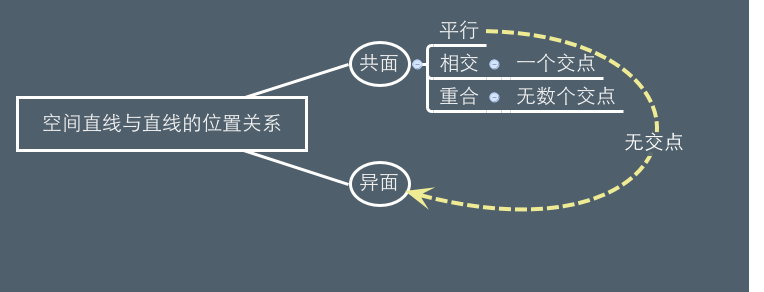
\includegraphics[height=100px]{/Users/shuyue/Desktop/1.png}


\geometry{a4paper} 

\begin{document}
\begin{CJK}{UTF8}{gkai}

\title{空间直线与直线的位置关系(异面直线)}
\date{}
\author{张舒悦}
\maketitle

\section{教学目标}
\begin{enumerate}
\item 
\item 
\item 
\end{enumerate}

\section{教学重点}
\begin{enumerate}
\item 
\item 
\item 
\end{enumerate}

\section{教学难点}
\begin{enumerate}
\item 
\item 
\item 
\end{enumerate}

\section{教学过程}
%\begin{multicols}{2}
%1\columnbreak \\ 2
%\end{multicols}
%\textcircled{1}
\subsection{引入}
\subsubsection{}
\subsubsection{}

\subsection{}
\subsection{}

\subsection{小结}
\begin{itemize}
\item
\item
\item
\item 
\end{itemize}

\subsection{思考题}
\begin{itemize}
\item
\item
\item
\item 
\end{itemize}

\subsection{作业}
\begin{enumerate}
\item 
\item
\item
\item
\end{enumerate}

\subsection{板书设计}
\begin{enumerate}
\item 
\item
\item
\item
\end{enumerate}



\end{CJK}
\end{document}